\documentclass{article}

\usepackage[magyar]{babel}
\usepackage{t1enc}
\usepackage{graphicx}
\usepackage{hulipsum}
\usepackage{enumitem}
\usepackage{subcaption}

\begin{document}
\begin{enumerate}
\item 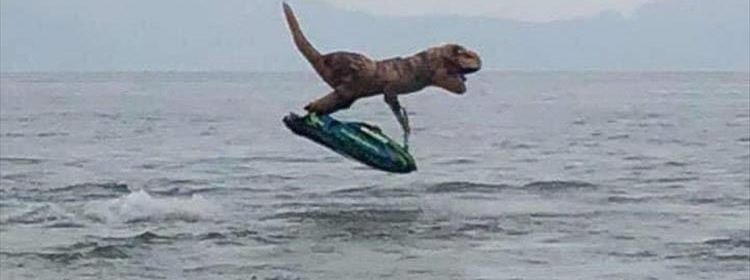
\includegraphics[width=5cm]{forras/image1}
\begin{enumerate}
\item 
\includegraphics[width=5cm]{forras/image2}
\begin{enumerate}
\item 
\includegraphics[width=5cm]{forras/image3}
\end{enumerate}
\end{enumerate}
\end{enumerate}
\hulipsum{1}
\begin{figure}[bt]
\centering
\caption{IZIRÁJDER ÖCSÉM}
\begin{subfigure}[c]{5cm}
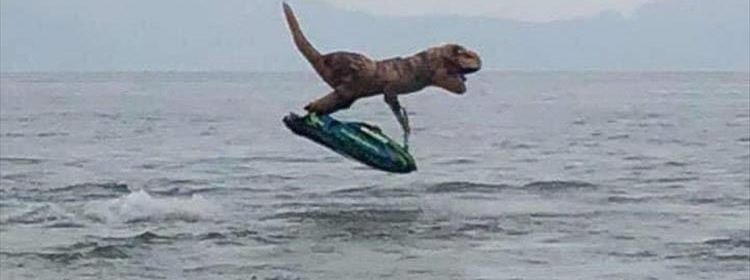
\includegraphics[width=5cm]{forras/image1}
\caption{anyád}
\end{subfigure}
\caption{IZIRÁJDER ÖCSÉM}
\caption{IZIRÁJDER ÖCSÉM}
\scalebox{-1}[-1]{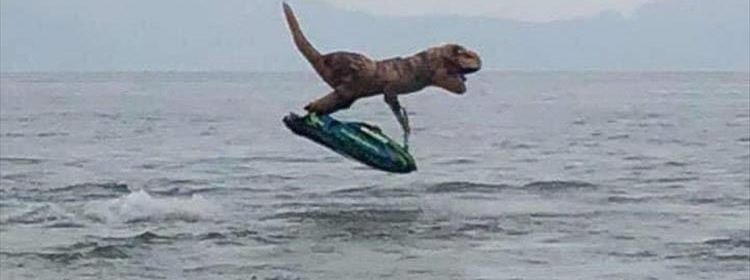
\includegraphics[width=5cm]{forras/image1}}
\end{figure}
\end{document}